\begin{figure}[H]
  \centering
  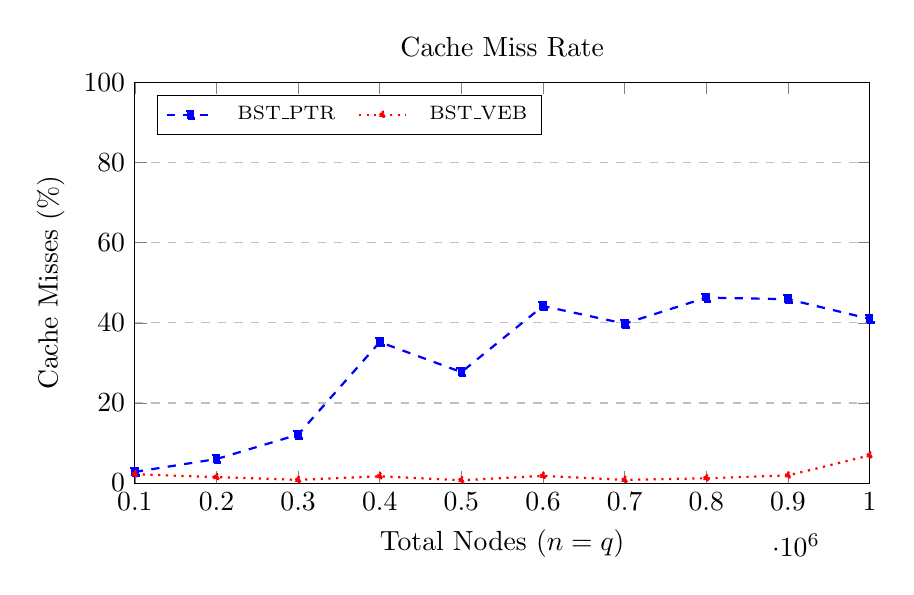
\begin{tikzpicture}
    \begin{axis}[
        title={Cache Miss Rate},
        xlabel={Total Nodes ($n=q$)},
        ylabel={Cache Misses (\%)},
        width =0.9\textwidth,
        height=0.55\textwidth,
        xmin=100000, xmax=1000000,
        ymin=0, ymax=100,
        ymajorgrids,
        grid style=dashed,
        legend columns=2,
        legend pos     = north west,
        legend style={font=\scriptsize, column sep=6pt},
    ]

    \addplot+[blue, thick, dashed, mark=square*, mark options={scale=.7,fill=blue}]
      coordinates {
        (100000,2.8) (200000,6.0) (300000,12.1) (400000,35.2)
        (500000,27.7) (600000,44.2) (700000,39.8) (800000,46.3)
        (900000,45.9) (1000000,41.0)
      };
    \addlegendentry{BST\_PTR}

    \addplot+[red, thick, dotted, mark=triangle*, mark options={scale=.7,fill=red}]
      coordinates {
        (100000,2.2) (200000,1.5) (300000,0.8) (400000,1.7)
        (500000,0.7) (600000,1.8) (700000,0.8) (800000,1.2)
        (900000,1.9) (1000000,6.9)
      };
    \addlegendentry{BST\_VEB}

    \end{axis}
  \end{tikzpicture}
  \caption{Cache miss rate (\%) as a function of total nodes and lookups ($n = q$) for the pointer-based (\texttt{BST\_PTR}) and VanEmde-Boas (\texttt{BST\_VEB}) implementations.}
  \label{fig:cachemiss}
\end{figure}
